\documentclass[10pt,a4paper]{article}
\usepackage[utf8]{inputenc}
\usepackage{amsmath}
\usepackage{gensymb}
\usepackage{amsfonts}
\usepackage{siunitx}
\usepackage[european]{circuitikz}
\usepackage{geometry}
\newgeometry{tmargin=2cm, bmargin=2cm, lmargin=2cm, rmargin=2cm}
\usepackage{amssymb}
\usepackage{multirow}
\usepackage{polski}
\usepackage{graphicx}
\author{\textbf{T. Fąs}}
\title{\textbf{BADANIE DIOD PÓŁPRZEWODNIKOWYCH}}
\begin{document}
\maketitle

\begin{center}
\textbf{\subsection*{STRESZCZENIE}}
\end{center}
W doświadczeniu badano charakterystyki prądowo-napięciowe diod krzemowych i LED, ich napięcie przewodzenia jak i napięcie przewodzenia oraz przebicia dla diod Zenera. Otrzymane wartości napięć przewodzenia były zgodne z wartościami rzeczywistymi, z kolei charakterystyki prądowa-napięciowe odbiegały od modelu teoretycznego.


\begin{center}
\textbf{\subsection*{WSTĘP}}
\end{center}
Diody półprzewodnikowe są obiektem zdolnym do przewodzenia prądu tylko w jednym kierunku. Natężenie prądu $I_{D}$ przepływającego przez diodę zależy od napięcia na diodzie $U_{D}$ według wzoru:
\begin{equation}
I_{D}=I_{G}\left[\exp{\left(\dfrac{eU_{D}}{MkT}\right)}-1\right],
\end{equation}
gdzie $e$ - ładunek elementarny, $k$ - stała Boltzmanna, $T$ - temperatura diody w kelwinach, $I_{G}$ - prąd generacji, a $M$ to stała charakteryzująca diodę. Znając wartości $I_{D}$ oraz $U_{D}$ można wyznaczyć wartość stałej $M$. 

Dodatkowo z diodami związane jest napięcie przewodzenia; jest to taka wartość napięcia $U_{D}$, po przekroczeniu której następuje gwałtowny wzrost natężenia prądu $I_{D}$. Dla diod Zenera wyróżnia się jeszcze napięcie Zenera $U_{Z}$, którego przyłożenie powoduje przebicie diody i przepływ prądu w kierunku przeciwnym do kierunku przewodzenia diody.

Na Rysunku 1 i Rysunku 2 przedstawiono charakterystyki prądowo-napięciowe dla diody krzemowej i Zenera.

\begin{figure}[h!]
\centering
\begin{minipage}{0.5\textwidth}
  \centering
  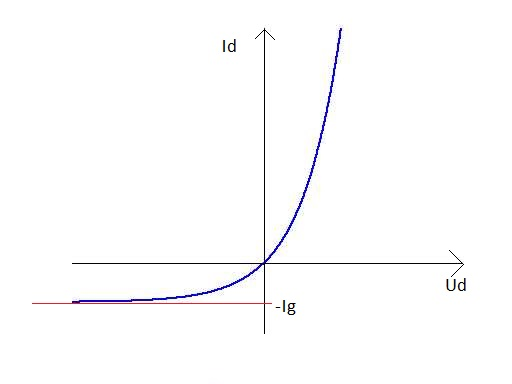
\includegraphics[width=8cm, height=5cm ]{rap20rys1} 
\caption{Charakterystyka diody krzemowej.}
\end{minipage}%
\begin{minipage}{0.5\textwidth}
  \centering
  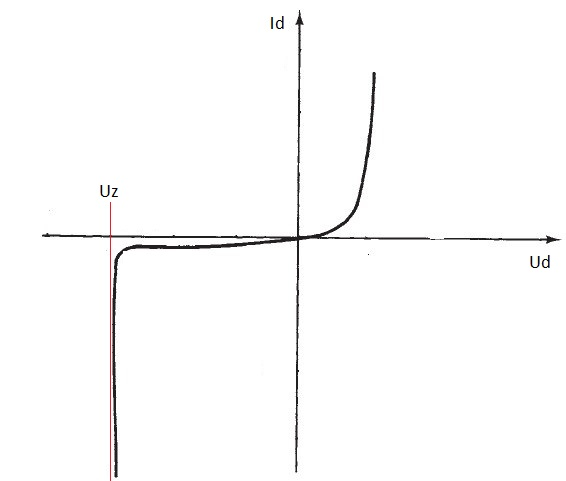
\includegraphics[width=8cm, height=5cm ]{rap20rys2} 
\caption{Charakterystyka diody Zenera.}
\end{minipage}
\end{figure}

W doświadczeniu zmierzono wartości $U_{D}$ oraz $I_{D}$, dla diody krzemowej i LED i na tej podstawie wyrysowano ich charakterystyki prądowo-napięciowe. Dla tych diod oszacowano napięcia przewodzenia, a dla diod Zenera dodatkowo oszacowano napięcie Zenera. Dodatkowo badano reakcje diod LED na zwiększanie amplitudy napięcia, jak i na zmiany częstości prądu.

\begin{center}
\textbf{\subsection*{UKŁAD DOŚWIADCZALNY}}
\end{center}
Układ doświadczalny składał się z oscyloskopu, generatora sygnałów, dwóch diod krzemowych, dwóch diod LED, dwóch diod Zenera oraz z dwóch oporników i płytki drukowanej. Zbudowano układ taki jak na Rysunku 3, przy czym diody przedstawione na schemacie były zmieniane w zależności od potrzeb. Tak przygotowany obwód podłączono do oscyloskopu i generatora według Rysunku 4. Pomiary na oscyloskopie wykonywano w trybie XY.


\begin{figure}[h!]
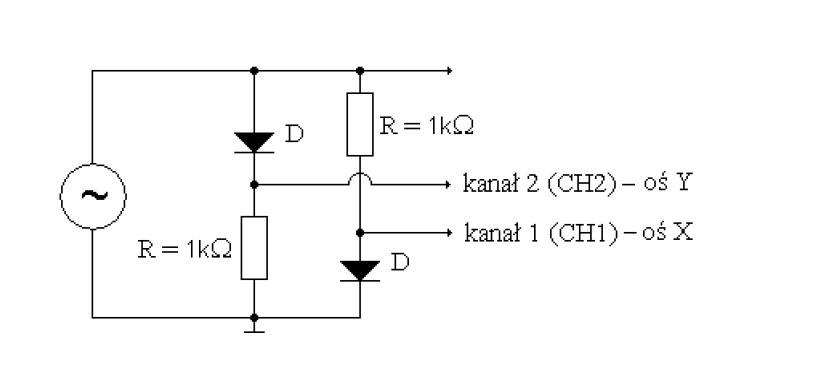
\includegraphics[width=10cm]{rap20rys11} 
\centering
\caption{Schemat obwodu \cite{r2}.}
\end{figure}


\begin{figure}[h!]
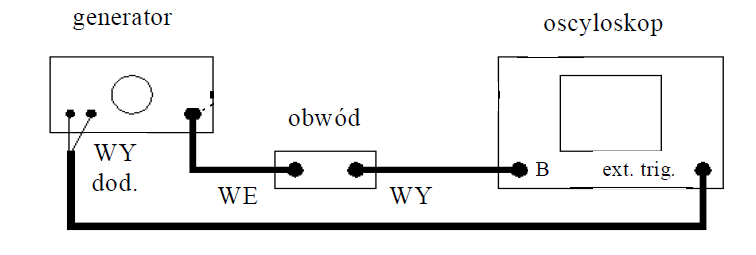
\includegraphics[width=10cm]{rap20rys22} 
\centering
\caption{Schemat układu \cite{r1}.}
\end{figure}

\begin{center}
\textbf{\subsection*{WYNIKI POMIARÓW}}
\end{center}
Zamiast natężenia $I_{D}$ zmierzono wartość napięcia na oporniku o $R=1010,25$ $\Omega$. Zmierzone napięcie to po prostu iloczyn $I_{D}$ oraz $R$. Otrzymane wartości $U_{D}$ oraz $I_{D}R$ dla diod krzemowych i świecących LED przedstawiono w Tabeli 1. Pomiary przeprowadzono dla prądu o napięciu 5 V i częstości 100 Hz dla diod krzemowych oraz 8 V i 1 Hz dla diod LED. 

\begin{table}[h!]
\centering
\caption{Wyniki pomiarów.}
\begin{tabular}{|c|c|c|c|c|c|c|c|}
\hline
\multicolumn{4}{|c|}{Diody krzemowe}                    & \multicolumn{4}{c|}{Diody LED}                          \\ \hline
$U_{D}$ [V] & $I_{D}R$ [V] & $U_{D}$ [V] & $I_{D}R$ [V] & $U_{D}$ [V] & $I_{D}R$ [V] & $U_{D}$ [V] & $I_{D}R$ [V] \\ \hline
0,52        & 0,26         & 0,58        & 1,72         & 1,68        & 2,147        & 1,54        & 0,176        \\ \hline
0,54        & 0,87         & 0,57        & 1,33         & 1,67        & 2,09         & 1,52        & 0,088        \\ \hline
0,5         & 0,22         & 0,48        & 0,19         & 1,65        & 1,716        & 1,5         & 0,082        \\ \hline
0,46        & 0,14         & 0,44        & 0,15         & 1,63        & 1,397        & 1,48        & 0,077        \\ \hline
0,38        & 0,07         & 0,34        & 0,05         & 1,6         & 0,54         & 1,62        & 1,507        \\ \hline
0,4         & 0,06         & 0,59        & 1,77         & 1,58        & 0,66         & 1,66        & 1,991        \\ \hline
0,53        & 0,44         & 0,56        & 1            & 1,56        & 0,297        & 1,6         & 0,704        \\ \hline
\end{tabular}
\end{table}
 
 Zmierzone bezpośrednio oraz oszacowane z charakterystyki prądowo-napięciowej wartości napięcia przewodzenia zgromadzono w Tabeli 2. W ostatniej kolumnie wypisano napięcia Zenera dla diod Zenera.
 
\begin{table}[h!]
\centering
\caption{Wartości napięć przewodzenia i napięcia Zenera [V]}
\begin{tabular}{|c|c|c|c|c|}
\hline
Dioda:                     & Krzemowa & LED  & Zenera & Napięcie Zenera \\ \hline
\multirow{2}{*}{Zmierzone} & 0,575    & 1,60 & 0,735  & 1,957           \\ \cline{2-5} 
                           & 0,575    & 1,60 & 0,735  & 1,907           \\ \hline
Z charakterystyki          & 0,570    & 1,52 & 0,720  & 1,800           \\ \hline
\end{tabular}
\end{table}
 
Kolejne pomiary dotyczyły badania zachowania diod LED na zmiany napięcia. Dodawanie stałego napięcia zwiększało jasność diod, a dla napięcia o wartości 10 V zaczynają świecić stale przy napięciu pierwotnym o amplitudzie 4 V i częstości 1 Hz. Diody przestają świecić przy stałym członie wynoszącym -3 V.
 
 Następnie zbadano, dla jakich częstości napięcia diody świecą stale. W pierwszej kolejności zwiększano częstość, dopóki diody nie zaczęły świecić stale, a w drugim pomiarze zaczęto od wysokiej częstości i zaczęto ją zmniejszać, dopóki nie dotowano pulsacji światła. Dla napięcia o amplitudzie 8 V i zerowym członie stałym częstości te wynosiły kolejno 33 Hz i 32 Hz.
 
\begin{center}
\textbf{\subsection*{ANALIZA DANYCH}}
\end{center}

Szybki rzut oka na dane z Tabeli 2 pozwala stwierdzić, iż wartości te są ze sobą zgodne. Zgodność tych wyników zadowala tym bardziej, jeśli weźmie się pod uwagę fakt, że pomiary na oscyloskopie cechowały się wysoką niedokładnością.


Do danych z Tabeli 1 dopasowano krzywą o wzorze zadanym Równaniem (1). Założone, że $T=300$ K, tak więc jedynymi parametrami dopasowania były $I_{G}$ oraz $M$. Ze względu na wysoką niedokładność pomiarów założono, że niepewność pomiarów $I_{D}$ wynosi 10\%. Otrzymane krzywe przedstawiono na Rysunku 5 I Rysunku 6, a parametry dopasowania przedstawiono w Tabeli 3.

\begin{figure}[h!]
\includegraphics[width=14cm]{rap20rys3} 
\centering
\caption{Krzywa najlepszego dopasowania: diody krzemowe.}
\end{figure}


\begin{figure}[h!]
\includegraphics[width=14cm]{rap20rys4} 
\centering
\caption{Krzywa najlepszego dopasowania: diody LED.}
\end{figure}

\begin{table}[h!]
\centering
\caption{Parametry dopasowania.}
\begin{tabular}{|c|c|c|c|c|}
\hline
Dioda    & $I_{G}$ [nA]       & Niepewność $I_{G}$ [nA] & $M$ & Niepewność M \\ \hline
Krzemowa & 6,5                & 9,2                     & 1,8 & 1,9          \\ \hline
LED      & 3,5$\cdot 10^{-9}$ & 6,3$\cdot 10^{-9}$      & 1,9 & 1,9          \\ \hline
\end{tabular}
\end{table}
Wartości $chi^2$ wynoszą kolejno 54,82 i 21,33 dla diod krzemowych i LED. Obie te wartości są powyżej wartości krytycznej 21,03, tak więc na podstawie testu $\chi^2$ nie można uznać tych krzywych za zgodne z danymi.


Przyglądając się obu wykresom, to dopasowanie dla diod krzemowych można byłoby uznać za w miarę zgodne, jednakże dopasowanie  dla diod LED jest kompletnie niezgodne z pomiarami i nie może być uznane za zgodne z przewidywaniami. Wydaję się to być sprzeczne z otrzymanymi wartościami $\chi^2$. Pomimo tego, że na ekranie oscyloskopu rysował się kształt z Rysunku 1, to zmierzenie dokładnych wartości napięć okazało się zbyt trudne. Rozdzielczość oscyloskopu w trybie XY była niewystarczająca na tego typu pomiary.


\begin{figure}[h!]
\includegraphics[width=14cm]{rap20rys6} 
\centering
\caption{Krzywa najlepszego dopasowania: diody krzemowe.}
\end{figure}


\begin{figure}[h!]
\includegraphics[width=14cm]{rap20rys5} 
\centering
\caption{Krzywa najlepszego dopasowania: diody LED.}
\end{figure}



  Na Rysunku 7 i Rysunku 8 przedstawiono te same wykresy w postaci logarytmicznej. Ma tutaj miejsce ciekawa rzecz: wykres dla diod LED zdaje się być lepiej dopasowany od wykresu dla diod krzemowych. 
Jednak zachowanie to dziwi mniej, kiedy weźmie się pod uwagę wartości $\chi^2$. Tak więc na podstawie wykresów logarytmicznych oraz wartości $\chi^2$ można uznać otrzymaną charakterystykę prądowo-napięciową dla diod LED za zgodną z przewidywaniami, z kolei charakterystyki dla diod krzemowych nie można za takową uznać; nastąpiła zbyt duża rozbieżność wyników. 





\begin{center}
\textbf{\subsection*{DYSKUSJA WYNIKÓW I WNIOSKI}}
\end{center} 

Otrzymane wartości napięć przewodzenia oraz napięć Zenera są ze sobą zgodne. Jednakże otrzymane charakterystyki pozastawiają wiele do życzenia. O tyle, o ile charakterystykę diod LED można jeszcze uznać, usprawiedliwiając się niedokładnością oscyloskopu, to w przypadku charakterystyki diod krzemowych takie usprawiedliwienie nie wystarczy. Należałoby wykonać ponowny pomiar na sprzęcie o lepszej rozdzielczości, aby móc ocenić, czy dane diody podlegają Równaniu (1). 






\begin{center}
\begin{thebibliography}{9}

\bibitem{r2}
 Praca zbiorowa,
 \emph{Instrukcja do ćwiczenia "Dioda półprzewodnikowa"},
 FUW, Warszawa, 2016, s. 1.
 
 
 \bibitem{r1}
 Praca zbiorowa,
 \emph{Instrukcja do ćwiczenia "Badanie szeregowego filtru rezonansowego RLC"},
 FUW, Warszawa, 2018, s. 2.
 

 
 \end{thebibliography}

\end{center}


\end{document}